\documentclass[a4paper,10pt,ngerman]{scrartcl}
\usepackage{babel}
\usepackage[T1]{fontenc}
\usepackage[utf8x]{inputenc}
\usepackage[a4paper,margin=2.5cm,footskip=0.5cm]{geometry}

% Die nächsten drei Felder bitte anpassen:
\newcommand{\Aufgabe}{Aufgabe 1: \LaTeX-Dokument} % Aufgabennummer und Aufgabennamen angeben
\newcommand{\TeilnahmeId}{?????}                  % Teilnahme-ID angeben
\newcommand{\Name}{Vor- und Nachname}             % Name des Bearbeiter / der Bearbeiterin dieser Aufgabe angeben

% Kopf- und Fußzeilen
\usepackage{scrlayer-scrpage, lastpage}
\setkomafont{pageheadfoot}{\large\textrm}
\lohead{\Aufgabe}
\rohead{Teilnahme-ID: \TeilnahmeId}
\cfoot*{\thepage{}/\pageref{LastPage}}

% Position des Titels
\usepackage{titling}
\setlength{\droptitle}{-1.0cm}

% Für mathematische Befehle und Symbole
\usepackage{amsmath}
\usepackage{amssymb}

% Für Bilder
\usepackage{graphicx}

% Für Algorithmen
\usepackage{algpseudocode}

\usepackage{caption}
\usepackage{subcaption}

\usepackage{tabularx}
\usepackage{booktabs}
\usepackage{amsthm}
% Für Quelltext
\usepackage{listings}
\usepackage{color}
\definecolor{mygreen}{rgb}{0,0.6,0}
\definecolor{mygray}{rgb}{0.5,0.5,0.5}
\definecolor{mymauve}{rgb}{0.58,0,0.82}
\lstset{
  keywordstyle=\color{blue},commentstyle=\color{mygreen},
  stringstyle=\color{mymauve},rulecolor=\color{black},
  basicstyle=\footnotesize\ttfamily,numberstyle=\tiny\color{mygray},
  captionpos=b, % sets the caption-position to bottom
  keepspaces=true, % keeps spaces in text
  numbers=left, numbersep=5pt, showspaces=false,showstringspaces=true,
  showtabs=false, stepnumber=2, tabsize=2, title=\lstname
}
\lstdefinelanguage{JavaScript}{ % JavaScript ist als einzige Sprache noch nicht vordefiniert
  keywords={break, case, catch, continue, debugger, default, delete, do, else, finally, for, function, if, in, instanceof, new, return, switch, this, throw, try, typeof, var, void, while, with},
  morecomment=[l]{//},
  morecomment=[s]{/*}{*/},
  morestring=[b]',
  morestring=[b]",
  sensitive=true
}

% Diese beiden Pakete müssen zuletzt geladen werden
%\usepackage{hyperref} % Anklickbare Links im Dokument
\usepackage{cleveref}

% Daten für die Titelseite
\title{\textbf{\Huge\Aufgabe}}
\author{\LARGE Teilnahme-ID: \LARGE \TeilnahmeId \\\\
  \LARGE Bearbeiter/-in dieser Aufgabe: \\
  \LARGE \Name\\\\}
\date{\LARGE\today}
\newtheorem{theorem}{Satz}
\newtheorem{lemma}[theorem]{Lemma}

\begin{document}

\maketitle
\tableofcontents

\vspace{0.5cm}

\section{Lösungsidee}
\subsection{Notation}
Mit "Stapel" ist im Folgenden immer der Begriff der Aufgabenstellung gemeint,
nicht die Datenstruktur. Die Menge der möglichen Stapel der Höhe $n$ wird mit
$\mathsf{P}_n$ bezeichnet. Die Möglichen Pfannkuchen-Wende-und-Ess-Operationen
für einem Stapel mit $n$ Pfannkuchen wird mit $\mathsf{W}_n$ bezeichnet. Die
Menge der möglichen Umkehroperationen für solch einen Stapel wird mit
$\mathsf{W}^{-1}_n$ bezeichnet. Wenn der Stapel $S \in \mathsf{P}_n$ durch die
Operation $w \in \mathsf{W}_n$ verändert wird, so wird der neue Stapel $S' = w
  S$ bezeichnet. Operationen assoziieren nach rechts, d.h. $w_1 w_2 S = w_1 (w_2
  S)$. Die Funktionen $A$ und $P$ werden aus der Aufgabenstellung übernommen.
Wird ein Stapel im Text dargestellt, dann steht der erste Pfannkuchen für den
obersten, der zweite für den zweitobersten und so weiter. Pfannkuchenstapel
werden entweder in Klammern durch Kommas getrennt (z.B. $(2,7,1,8)$) oder als
nicht getrennte Ziffern dargestellt (z.B. $2718$). Bei der zweiten Notation
können Pfannkuchen dann maximal die Breite 9 haben, um die Eindeutigkeit der
Darstellung zu gewährleisten.
\subsection{Sortieren}
\begin{figure}[t]
  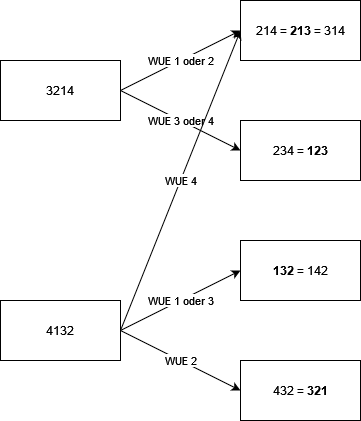
\includegraphics[scale=0.5]{pancakegraph}
  \centering
  \caption{Ausschnitt aus dem Graph der Pfannkuchenstapel. Die Kanten sind beschriftet mit der zugehörigen Operation.}
\end{figure}
Die möglichen Stapel können in einem gerichteten Graphen dargestellt werden (Siehe Abbildung 1). Die Knoten des Graphen
sind die Stapel, die Kanten sind die Operationen. Die Kanten sind gerichtet, denn eine PWUE-Operation
wandelt einen Stapel in einen anderen um. Die Identität eines Stapels wird durch die Reihenfolge der Pfannkuchen bestimmt,
nicht deren genauen Größen. Das heißt, dass zum Beispiel die Stapel $(10,12,3)$ und $(2,3,1)$ gleich sind, denn die Elemente haben die gleiche
Reihenfolge. Das hängt damit zusammen, dass der Zielstapel nur durch seine aufsteigende Reihenfolge definiert ist. Äquivalente Stapel können
in eine kanonische Form gebracht werden, in dem die kleinste Größe durch 1, die zweitkleinste durch 2 und so weiter ersetzt werden. Dadurch ist
$(2,3,1)$ in kanonischer Form. Die kanonische Form kann folgendermaßen bestimmt werden:
\begin{algorithmic}
  \Procedure{Kanonische Form}{Stapel $S$}
  \State{Initialisiere Integer-Array $V$ der Länge $\max(S) - \min(S) + 1$}
  \State{Setze jeden Wert von $V$ auf $-1$}
  \For{$s \in S$}
  \State{$V_{s - \min(S)} \gets 1$}
  \EndFor
  \State{Initalisiere Zähler $c=1$}

  \For{$s \in (0, 1, \ldots, |V|-1)$}
  \If{$V_s \neq -1$}
  \State{$V_s \gets c$}
  \State{$c \gets c+1$}
  \EndIf
  \EndFor
  \State{Initalisiere Integer-Array $E$ der Länge $|S|$}
  \For{$s \in (0, 1, \ldots, |S|-1)$}
  \State{$E_s \gets V_{s-\min(S)}$}
  \EndFor

  \Return{$E$}
  \EndProcedure
\end{algorithmic}
Dieser Algorithmus konstruiert im Array $V$ eine Abbildung der Zahlenwerte der ursprünglichen Pfannkuchen in
jene der kanonischen Form, wobei der Array-Index den Parameter der Abbildung darstellt. Dafür wird zunächst jeder
Index, der zu einer Breite im ursprünglichen Stapel gehört, markiert. Die markierten Indices werden dann aufsteigend
nummeriert, der kleinste bekommt also den Wert $1$, der zweitkleinste $2$ und so weiter. So ist die Konstruktion
der Abbildung vollständig. Im letzten Schritt wird die Abbildung auf die Elemente von $S$ angewandt. Da die Abbildung
nur für bestimmte Werte zwischen einschließlich dem kleinsten und größten von $S$ definiert ist, kann die Länge des Arrays
auf $\max(S)-\min(S)$ begrenzt werden. Für die Abbildung muss deshalb immer noch $\min(S)$ vom Parameter abgezogen werden.
\\\\
Um die Operationen zu bestimmen, die einen Stapel optimal sortieren, muss
ein kürzester Pfad im Graphen vom Stapel zu einem sortierten Stapel gefunden werden. Dafür lässt sich
Dijkstra's Algorithmus \cite{dijkstra_1959} verwenden.
\begin{algorithmic}
  \Procedure{Dijkstra's Algorithmus}{Stapel $S$}
  \State{Intialisiere Prioritätswarteschlange $Q$}
  \State{Initialisiere Map $V$}
  \State{Initialisiere Map $C$}
  \State{Füge $S$ mit Priotität $0$ in $Q$ ein}
  \State{Füge $S$ mit Vorgänger $()$ in $V$ ein}
  \State{Füge $S$ mit Kosten $0$ in $C$ ein}
  \While{$Q$ nicht leer}
  \State{Entferne Knoten $S$ mit der niedrigsten Priorität aus $Q$}
  \If{$S$ ist sortiert}
  \State{Rekonstruiere Pfad von $S$ zu $()$ mit $V$}
  \EndIf
  \For{alle $w \in \mathsf{W}_n$}
  \State{$S' \gets w S$}
  \State{$k \gets C(S) + 1$}
  \If{$S'$ nicht in $C$ oder $K < C(S')$}
  \State{Füge $S'$ mit Priorität $k$ in $Q$ ein}
  \State{Füge $S'$ mit Vorgänger $S$ in $V$ ein}
  \State{Füge $S'$ mit Kosten $k$ in $C$ ein}
  \EndIf
  \EndFor
  \EndWhile
  \EndProcedure
\end{algorithmic}
Dieser Algorithmus hat außer der Länge der Permutationskette keine Informationen über die Stapel.
Da Dijkstras Algorithmus alle kürzeren erkundeten Pfade erweitert bevor ein längerer Pfad erweitert
wird, ist er hier sehr langsam. Schnellere Ergebnisse lassen sich mit Hilfe vom A*-Algorithmus \cite{hart_1968} erreichen.
Dieser Algorithmus ähnelt Dijkstras Algorithmus, verwendet aber eine Heuristik, welche die Distanz zum
Ziel schätzt. Die Heuristik darf die tätsächliche Entferung zum Ziel niemals überschätzen. Mit $H(S)$ als Heuristik
für den Stapel $S$ lautet der Algorithmus:\\\\
\begin{algorithmic}
  \Procedure{A*-Algorithmus}{Stapel $S$}
  \State{Intialisiere Prioritätswarteschlange $Q$}
  \State{Initialisiere Map $V$}
  \State{Initialisiere Map $C$}
  \State{Füge $S$ mit Priotität $0$ in $Q$ ein}
  \State{Füge $S$ mit Vorgänger $()$ in $V$ ein}
  \State{Füge $S$ mit Kosten $0$ in $C$ ein}
  \While{$Q$ nicht leer}
  \State{Entferne Knoten $S$ mit der niedrigsten Priorität aus $Q$}
  \If{$S$ ist sortiert}
  \State{Rekonstruiere Pfad von $S$ zu $()$ mit $V$}
  \EndIf
  \For{alle $w \in \mathsf{W}_n$}
  \State{$S' \gets w S$}
  \State{$k \gets C(S) + 1 - H(S) + H(S')$}
  \If{$S'$ nicht in $C$ oder $K < C(S')$}
  \State{Füge $S'$ mit Priorität $k$ in $Q$ ein}
  \State{Füge $S'$ mit Vorgänger $S$ in $V$ ein}
  \State{Füge $S'$ mit Kosten $k$ in $C$ ein}
  \EndIf
  \EndFor
  \EndWhile
  \EndProcedure
\end{algorithmic}
Eine Heuristik für das Pfannkuchen sortieren ist die Anzahl der Adjazenzen \cite{gates_1979}. Als Adjazenz bezeichne ich zwei
Pfannkuchen die direkt nebeneinander im Stapel liegen und für die es keinen Pfannkuchen gibt, dessen Größe zwischen den beiden liegt.
Mit Hilfe der Adjazenzen lässt sich eine untere Schranke für die Anzahl der Sortierschritte eines Stapels berechnen.
\begin{lemma}
  Ein Stapel der Höhe $h$ mit $a_0$ Adjazenzen kann in nicht weniger als $\lceil\frac{h - a_0}{3}\rceil$ Schritten sortiert werden.
\end{lemma}
\begin{proof}
  In einer Operation können sich höchstens zwei neue Adjazenzen bilden. Weil in einer Operation sich nur die Nachbarn von zwei
  Pfannkuchen ändern, (nämlich des obersten, der nach unten gewendet wird, und dessen, der direkt unter dem Pfannenwender liegen bleibt)
  kann sich nur zwischen diesen beiden eine Adjazenz bilden. Eine weitere Adjazenz lässt sich dadurch bilden, dass der aufgegessene
  Pfannkuchen die Breite zwischen zwei nebeneinanderliegenden hatte, welche nach der Operation keine Pfannkuchen mit Größe zwischen ihnen haben.
  Als Ajdazenz wird auch gezählt, wenn der größte Pfannkuchen ganz unten liegt. Ein sortierter Stapel der Höhe $n$ hat $n$ Adjazenzen.
  Seien $a_0$ die Anzahl der Adjazenzen im untersuchten Stapel, $h$ die Höhe des Stapels und $n$ die Anzahl der Sortieroperationen. Weiterhin seien
  $a_f$ und $h_f$ die Anzahl der Adjazenzen und die Höhe des sortierten Stapels. Dann gilt:
  \begin{align*}
    I.              &  & a_f      & = h_f                              & \text{Adjazenzen und Höhe des Stapels müssen gleich sein}            \\
    II.             &  & a_f      & \leq a_0 + 2n                      & \text{Pro Operation können höchstens zwei neue Adjazenzen entstehen} \\
    III.            &  & h_f      & = h - n                            & \text{Der Stapel wird in jedem Schritt um einen Pfannkuchen kleiner} \\
    \noalign{II. und III. in I. einsetzen:}                                                                                                   \\
                    &  & a_0 + 2n & \geq h - n                         &                                                                      \\
    \leftrightarrow &  & n        & \geq \frac{h - a_0}{3}                                                                                    \\
    \noalign{Weil $n \in \mathbb{N}^+$ kann aufgerundet werden:}                                                                              \\
                    &  & n        & \geq \lceil\frac{h - a_0}{3}\rceil                                                                        \\
  \end{align*}
\end{proof}
Als untere Schranke kann diese Erkenntnis als für den A*-Algorithmus geeignete Heuristik verwendet werden,
mit $a(S)$ als Anzahl der Adjazenzen im Stapel $S$ und $h(S)$ als Höhe des Stapels $S$:
\begin{align*}
  H(S) = \lceil\frac{h(S) - a(S)}{3}\rceil
\end{align*}
\subsection{PWUE-Zahl}
Die PWUE-Zahl kann rekursiv mit Hilfe von dynamischer Programmierung berechnet
werden. Dafür definieren wir die Funktion $K(n,a)=\{s \in \mathsf{P}_n \mid
  A(s) = a\}$, die die Menge aller Stapel der Höhe $n$ enthält, die in mindestens
$a$ Schritten sortiert werden können. Die Funktion lässt sich rekursiv
berechnen:
\begin{align*}
  K(n,a) & = \{wS, w \in \mathsf{W}^{-1}_{n-1}, S \in K(n-1,a-1)\} | \forall v \in \mathsf{W}_n: A(vwS) \geq a-1\}                     \\
         & = \{wS, w \in \mathsf{W}^{-1}_{n-1}, S \in K(n-1,a-1)\} | \forall v \in \mathsf{W}_n: \exists b \geq a-1: A(vwS) = b\}      \\
         & = \{wS, w \in \mathsf{W}^{-1}_{n-1},S \in K(n-1,a-1)\} | \forall v \in \mathsf{W}_n: \exists b \geq a-1: vwS \in K(n-1,b)\} \\
\end{align*}
$K(n,a)$ enthält also alle Stapel, die durch eine Umkehroperation aus Stapeln der Höhe $n-1$ mit mindestens $a-1$ Sortieroperationen entstehen können
und für die keine andere Sortieroperation eine Stapel bildet, der in weniger als $a-1$ Schritten sortiert werden kann.
Nach dieser Definition würde $K(n, 1)$ allerdings auch die komplett sortierten Stapel enthalten, weshalb noch die Bedingung
$(a>1)\vee (s \notin K(n,0))$ ergänzt werden muss. Da die komplett sortierten Stapel nicht weiter sortiert werden müssen,
setzen wir $K(n,0) = \{(1, \dots, n)\}$, es handelt sich dabei um das Ende der Rekursion.
Die Funktion $K(n,a)$ ist also definiert als
\begin{align*}
  K(n,0) & = \{(1, \dots, n)\}                                                                                                                                             \\
  K(n,a) & = \{wS, w \in \mathsf{W}^{-1}_{n-1}, S \in K(n-1,a-1) | \forall v \in \mathsf{W}_n: \exists b \geq a-1: vwS \in K(n-1,b) \wedge ((a>1)\vee (S \notin K(n,0)))\} \\
\end{align*}
Dass diese Definition richtig ist, lässt sich überprüfen durch die Substitution
$A(S)=k, S \in \mathsf{P}_n \iff (\forall w \in \mathsf{W}_n: A(ws) \geq k-1)\wedge(\exists w \in \mathsf{W}_n: A(ws) = k-1)$.
Ein Problem bei der Berechnung dieser Funktion ist, dass $\exists b \geq a-1: vwS \in K(n-1,b) \wedge ((a>1)\vee (S \notin K(n,0)))$
nicht begrenzt ist, sondern alle natürlichen Zahlen durchprobieren müsste. Das ist natürlich Unfug, denn wir können nicht alle natürlichen
Zahlen in endlicher Zeit durchprobieren. Dass wir das nicht brauchen, zeigt folgendes Lemma:
\begin{lemma}
  Jeder Stapel der Höhe $3n+b$ mit $n,b\in \mathbb{N}$ und $b<3$ kann in weniger als oder gleich $2n+1$ Schritten sortiert werden.
\end{lemma}
\begin{proof}
  Wir beweisen durch starke Induktion nach $n$. Für $n=0$ kann der Stapel die Höhe $1$ oder $2$ haben. Im ersten Fall ist er Stapel schon sortiert
  und die Aussage ist erfüllt. Im zweiten Fall ist der Stapel sortiert oder noch falsch herum. In beiden Fällen ist nicht mehr als $2n+1=1$ Sortierschritt
  notwendig. \\
  Für einen Stapel mit $n>0$ liegen die $m$ größten Pfannkuchen in richtiger Reihenfolge ganz unten. Wenn $m\geq3$ muss somit nur der darüberliegende Stapel mit $3m+c;m<n$ Pfannkuchen
  sortiert werden. Das ist nach Induktion in $2m+1$ Schritten möglich, was kleiner als $2n+1$ ist, wodurch die Aussage erfüllt ist. Wenn $m<3$, können wir den $m+1$t-größten Pfannkuchen
  in einer Operation nach oben bringen und in einer zweiten an die richtige Stelle am Ende. Danach hat der unsortierte Teil des Stapels, also alles vor den letzten $m+1$ Pfannkuchen,
  die Höhe $3n+b-2-(m+1)=3n+b-3-m=3(n-1)+b-m$, weil zwei Pfannkuchen verspeist wurden und der sortierte Teil um einen größer geworden ist. Nach der Induktion kann dieser Teil der Höhe
  $3(n-1)+b-m$ in $2(n-1)+1$ Schritten sortiert werden. Zusammen mit den zwei Wendeoperationen wurde der Stapel in $2(n-1)+1+2=2n+1$ Schritten sortert.
\end{proof}
Es folgt sofort, dass für einen Stapel der Höhe $h$ gilt $n=\lfloor\frac{h}{3}\rfloor$ und dieser deshalb in $2\lfloor\frac{h}{3}\rfloor+1$ Schritten sortiert werden kann.
Allerdings lässt sich dadurch nicht direkt die PWUE-Zahl bestimmen, es handelt sich lediglich um eine obere Schranke für diese.
Da jeder Stapel $S \in \mathsf{P}_n$ in $2\lfloor\frac{h}{3}\rfloor+1$ Schritten sortiert werden kann, reicht es aus,
die Funktion $K(n,a)$ für alle $\lceil \frac{n}{1.5}\rceil$ zu berechnen.
Damit lässt sich auch $\exists b \geq a-1: vws \in K(n-1,b)$ durch $\exists \lceil \frac{n}{1.5}\rceil \geq b \geq a-1: vwS \in K(n-1,b)$
ersetzen, wodurch nicht unendlich viele Werte für $b$
ausprobiert werden müssen.
Um jetzt die PWUE-Zahl zu berechnen, muss nur noch die Funktion $K(n,a)$ für alle $a \leq 2\lfloor\frac{h}{3}\rfloor+1$
berechnet werden und überprüft werden, ob sie Elemente enthält:
\begin{algorithmic}
  \Procedure{PWUE-Zahl}{Höhe $h$}
  \State{Intitalisiere Map $\tilde{K}$}
  \State{Initialisiere Map $\tilde{S}$}
  \For{$i \in (2\lfloor\frac{h}{3}\rfloor+1, 2\lfloor\frac{h}{3}\rfloor, \ldots, 0)$}
  \If{$K(h, i) \neq \emptyset$}
  \Return{$i, K(h,i)$}
  \EndIf
  \EndFor
  \EndProcedure
  \Procedure{K}{Höhe $n$, Schritte $a$}
  \If{$\tilde{K}$ enthält Schlüssel $(n,a)$}
  \Return{$\tilde{K}[(n,a)]$}
  \EndIf
  \If{$a=0$}
  \State{$\tilde{K}[(n,a)] \gets (1, 2, \ldots, n)$}
  \State{$\tilde{S}[(1,2,\ldots, n)] \gets 0$}
  \Return{$\{(1,2,\ldots, n)\}$}
  \EndIf
  \If{$a>0 \wedge n=1$}
  \State{$\tilde{K}[(n,a)] \gets (1, 2, \ldots, n)$}
  \Return{$\{(1,2,\ldots, n)\}$}
  \EndIf
  \State{Initialisiere leere Menge $R$}
  \For{$w \in \mathsf{W}^{-1}_{n-1}, S \in K(n-1,a-1)$}
  \If{$\neg(a>1 \vee wS = (1, 2, \ldots, n))$}
  \State{continue}
  \EndIf
  \State{Initialisiere boolesche Variable $A$ mit wahr}
  \For{$v \in \mathsf{W}_n$}
  \If{$\tilde{S}$ enthält Schlüssel $vwS$}
  \If{$\tilde{S}[vwS]<a-1$}
  \State{$A \gets \text{falsch}$}
  \State{break}
  \Else
  \State{continue}
  \EndIf
  \EndIf
  \State{Initialisiere boolesche Variable $E$ mit falsch}
  \For{$b \in (a-1, a, \ldots, 2\lfloor\frac{h}{3}\rfloor+1)$}
  \If{$vwS \in K(n-1, b)$}
  \State{$E \gets \text{wahr}$}
  \State{break}
  \EndIf
  \EndFor
  \State{$A \gets A \wedge E$}
  \If{$\neg A$}
  \State{break}
  \EndIf
  \EndFor
  \If{$A$}
  \State{$R \gets R \cup \{wS\}$}
  \State{$\tilde{S}[wS] \gets a$}
  \EndIf
  \EndFor
  \State{$\tilde{K}[(n,a)] \gets R$}
  \Return{$R$}
  \EndProcedure
\end{algorithmic}
Dieser Algorithmus kann noch schneller gemacht werden, in dem in der Prozedur "PWUE-Zahl" für $K(n,a)$ nicht alle Elemente gesucht werden, sondern das
erste zurückgegeben wird, denn dort sind nicht alle Elemente von $K(n,a)$ notwendig, sondern irgendeines, falls es existiert. Die Aufgabenstellung lautet ja nur einen
Stapel zu finden, der in der größten Zahl von Schritten sortiert werden kann.
\section{Laufzeit und Speicherbedarf}
\subsection{Sortieren}
Der A*-Algorithmus hat für einen Graph mit Kanten $V$ und Knoten $E$ eine
Laufzeit in\footnote{Da die Landau-Symbole Mengen von Funktionen darstellen,
ist es mathematisch korrekt zu sagen, die Zeit (-funktion) ist in
$\mathcal{O}(f(x))$. In den Gleichungen weiter unten knüpfe ich an die
verbreitere Notation an, in der $\mathcal{O}(f(x))$ für einen anonymen
  Funktionsterm dieser Menge steht.} $\mathcal{O}(|E| \log |V|)$ und einen
  Speicherbedarf in $\mathcal{O}(V)$ \cite[654]{sedgewick_wayne_2011}. Wenn wir
  einen Ausgangsstapel der Höhe $h$ haben, sind die Knoten des zu untersuchenden
  Graphs $V = \overset{.}\cup_{n=1}^{h-1} \mathsf{P}_n$. Da es $n!$ Permutationen
  von $n$ Elementen gibt, ist $|V| = \sum_{n=1}^{h-1}n!$. Diese Summe ist in
$\mathcal{O}(h!)$:
  \begin{align*}
    |V|      & = \sum_{n=1}^{h-1}n!                                                                           \\
             & = (h-1)! \cdot (1 + \frac{1}{h-1} + \frac{1}{(h-1)(h-2)} + \ldots + \frac{1}{(h-1)!})          \\
             & = (h-1)! \cdot (1 + \mathcal{O}(1))                                                            \\
             & = \mathcal{O}((h-1)!)                                                                 & | \log \\
    \log |V| & = \mathcal{O}((h-1) \log (h-1))
  \end{align*}
  Von einem Knoten, der zu einem Stapel der Höhe $n$ gehört, gibt es maximal $n$ verschiedene PWUE-Operationen und somit auch maximal $n$ ausgehende Kanten. Das heißt
  \begin{align*}
    |E| & = \sum_{n=1}^{h-1} n \cdot |\mathsf{P}_n|                                                                             \\
        & = \sum_{n=1}^{h-1} n \cdot n!                                                                                         \\
        & = (h-1) \cdot (h-1)! \cdot (1 + \frac{h-2}{(h-1)^2} + \frac{h-3}{(h-1)^2(h-2)} + \ldots \frac{1}{(h-1) \cdot (h-1)!}) \\
        & = (h-1) \cdot (h-1)! \cdot (1 + \mathcal{O}(1))                                                                       \\
        & = \mathcal{O}((h-1) \cdot (h-1)!)                                                                                     \\
        & = \mathcal{O}(h!)
  \end{align*}
  Demnach wäre die Laufzeit $\mathcal{O}(h! \cdot (h-1) \cdot \log (h-1))$ und der Speicherbedarf $\mathcal{O}(h!)$. Leider ist das etwas zu kurz gedacht, denn
  in jedem Expansionsschritt des Algorithmus muss für jeden neuen Knoten noch die kanonische Form gebildet werden. Außerdem kann der zu erweiternde Knoten nicht direkt
  mit einem Zielknoten verglichen werden, sondern es muss geprüft werden, ob seine Pfannkuchen in aufsteigender Reihenfolge sind. Diese Prüfung nimmt pro Stapel eine Zeit in
$\mathcal{O}(h)$ in Anspruch, da jeder Pfannkuchen mit seinem Vorgänger verglichen wird und jeder Stapel nicht mehr als $h$ Pfannkuchen enthält, was zu $h$ Vergleichsoperationen führt.
  Im schlechtesten Fall wird maximal jeder der Knoten überprüft, das heißt diese Operation nimmt eine Zeit in $\mathcal{O}(h \cdot |V|) = \mathcal{O}(h!)$ in Anspruch. Dieser Term
  wächst langsamer als $h! \cdot (h-1) \cdot \log (h-1)$, die Zeit bleibt also in $\mathcal{O}(h! \cdot (h-1) \cdot \log (h-1) + h!) = \mathcal{O}(h! \cdot (h-1) \cdot \log (h-1))$. Die
  Prüfung auf Sortiertheit nimmt keinen zusätzlichen Speicher in Anspruch.\\
  Betrachten wir nun die Zeit, in der die Stapel in kanonische Form gebracht werden. Die benötigte Zeit liegt für einen Stapel liegt in $\mathcal{O}(h)$: Um $\min(S)$ und $\max(S)$ zu finden, muss der
  Stapel, der nicht mehr als $h$ Pfannkuchen enthält, durchgegangen werden. Dann wird der gleiche Stapel noch einmal durchgegangen, um die Werte im Array $V$ zu ändern, wo wieder nicht mehr als
$h$ Iterationen benötigt werden. Dann werden die Elemente des Array $V$ durchgegangen. Dieses hat die Länge $\max(S) - \min(S) + 1$. Diese Länge ist auch niemals größer als $h$, weil
  der größte Pfannkuchen die Breite $h$ und der kleinste die Breite $1$ hat. Zuletzt wird noch einmal $S$ durchgegangen, um die Abbildung anzuwenden. Diese Operation wird für jeden neu
  erkundeten Stapel durchgeführt, also für jede Kante. Insgesamt wird dadurch die Zeit $\mathcal{O}(h \cdot |V|) = \mathcal{O}(h \cdot (h-1)!) = \mathcal{O}(h!)$ benötigt, was auch langsamer
  als der schon ermittelte Term für die Zeit wächst und somit vernachlässigt werden kann. Der zusätzliche Speicherbedarf liegt in $\mathcal{O}(h)$ für das Array $V$, was auch vernachlässigbar ist.
  Die Kanonisierung eines Stapels der Höhe $h$ muss mindestens in $\mathcal{O}(n)$ liegen, da das Ergebnis der Länge $n$ ja ausgegeben muss. Da die Höhe der Stapel zu $h$ proportional ist,
  ist die Zeit $\mathcal{O}(h)$ meines Algorithmus somit optimal. \\
  Zusammenfassend ist die Zeit in $\mathcal{O}(h! \cdot (h-1) \cdot \log (h-1))$ und der Speicherbedarf in $\mathcal{O}(h!)$. \\
  \begin{figure}
    \centering
    \begin{subfigure}{.5\textwidth}
      \centering
      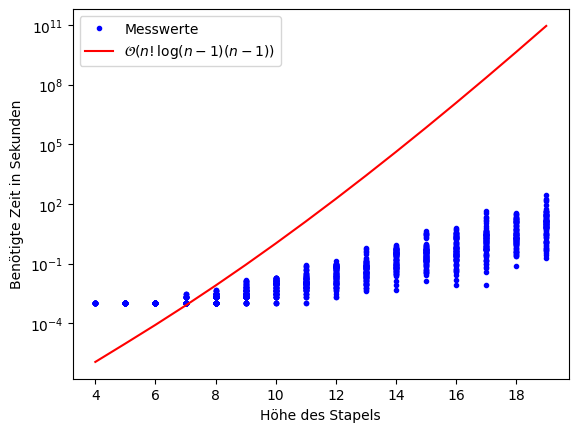
\includegraphics[width=1\linewidth]{zeit-hoehe-bigo.png}
      \caption{Messwerte zusammen mit Vorhersage}
      \label{fig:sub1}
    \end{subfigure}%
    \begin{subfigure}{.5\textwidth}
      \centering
      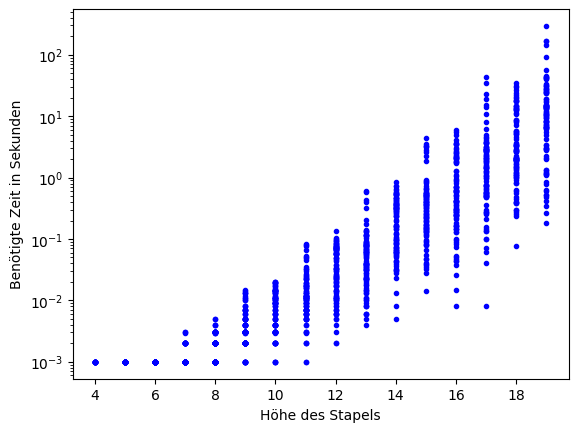
\includegraphics[width=1\linewidth]{zeit-hoehe.png}
      \caption{Messwerte allein}
      \label{fig:sub2}
    \end{subfigure}
    \caption{Die Diagramme zeigen die benötigte Zeit für jeweils 100 zufällige Stapel unterschiedlicher Höhen. Man bemerke die logarithmische Skala der Zeit.}
    \label{fig:test}
  \end{figure}
  Abbildung 2 zeigt, dass die tatsächliche Zeit zwar exponentiell wächst (lineares Wachstum auf einer logarithmischen Skala), wie man aber in Abbildung 2a sieht,
  ist die Steigung kleiner als die theoretische Analyse ergeben hat. Trotzdem scheint die Zeit in $\mathcal{O}(h! \cdot (h-1) \cdot \log (h-1))$ zu liegen, denn ab einem
  bestimmten Punkt ist die Zeit kleiner als eine Funktion dieser Menge.
  \subsection{PWUE-Zahl}
  Um $K(n,a)$ zu ermitteln, werden alle $S \in K(n-1, a-1), w \in
\mathsf{W}^{-1}_{n-1}, v \in \mathsf{W}_n$ durchgegangen.
$|\mathsf{W}^{-1}_{n-1}|=(n+1)^2$, weil wir $(n+1)$ verschiedene Pfannkuchen
  auf den Stapel legen können (den kleinsten, zweitkleinsten, ..., größten) und
  dann $(n+1)$ verschiedene Wendeoperationen durchführen können.
$|\mathsf{W}_n|=n$, weil wir nur den ersten Pfannkuchen wenden, die ersten zwei
  Pfannkuchen wenden, usw. können, bis wir alle $n$ Pfannkuchen wenden. \\ Da die
  Summe alle möglichen Permutationen umfassen muss, gilt:
  \begin{align*}
    \sum_{a=0}^{2\lfloor\frac{n}{3}\rfloor+1}|K(n,a)| & =n!
  \end{align*}
  Wenn wir nun für ein $n$ alle $K(n,a)$ berechnen, benötigen wir
  \begin{align*}
    \sum_{a=0}^{2\lfloor\frac{n}{3}\rfloor+1}|K(n-1,a-1)| \cdot |\mathsf{W}^{-1}_{n-1}| \cdot |\mathsf{W}_n|
     & = |\mathsf{W}^{-1}_{n-1}| \cdot |\mathsf{W}_n| \cdot \sum_{a=0}^{2\lfloor\frac{n}{3}\rfloor+1}|K(n-1,a-1)|
     & = (n+1)(n+1)n \cdot \sum_{a=0}^{2\lfloor\frac{n}{3}\rfloor+1}|K(n-1,a-1)|
     & = (n+1)(n+1)n\mathcal{O}((n-1)!)
     & = \mathcal{O}(n^3(n-1)!)
  \end{align*}
  Kombinationen. Da wir $n$ für alle $1 \leq n \leq h-1$ berechnen müssen, um die PWUE-Zahl zu ermitteln, werden insgesamt
  \begin{align*}
    \sum_{n=1}^{h-1}\mathcal{O}(n^3(n-1)!) & = \mathcal{O}(\mathcal{O}((h-1)^3(h-2)!) \cdot (h-1))
                                           & = \mathcal{O}(h^3(h-2)!)
  \end{align*}
  Kombinationen durchprobiert. Für eine Kombination wird eine Zeit in $\mathcal{O}(h)$ verwendet, da die Kanonisierung wie oben erläutert
  diese Zeit benötigt, und die Vergleichs- und Wendeoperationen so wie die Hashfunktionen der Hashmap-Datenstrukturen auch lineare Zeit benötigen.
  Die Zeit liegt also in $\mathcal{O}(h^4(h-2)!)$. Da auch alle Kombinationen gespeichert werden und eine Kombination Länge in $\mathcal{O}(h)$ hat,
  ist die Speicherkomplexität auch in $\mathcal{O}(h^4(h-2)!)$.
\section{Umsetzung}
Zur Lösung der ersten Aufgabe habe ich Python verwendet. Für die zweite Aufgabe
habe ich Java verwendet. Die Lösung der ersten Aufgabe verlangt einen Dateipfad
zum Pfannkuchenstapel. Diese Datei ist in dem Format, welches die
Beispieleingaben auf der BwInf-Webseite haben. Das Programm sucht die Lösung
und gibt dann die PWUE-Operationen sowie die Zwischenstände des Stapels aus.
Die Notation weicht etwas von der hier verwendeten ab, denn die einzelnen
Pfannkuchen werden nicht durch Kommata sondern durch Leerzeichen getrennt und
der Stapel ist nicht umklammert.
\section{Beispiele}
\subsection{Sortieren}
Die Beispiele \lstinline|pancake0.txt| bis \lstinline|pancake7.txt| sind direkt
von den BwInf-Webseiten übernommen. Die Beispiele \lstinline|pancake2h.txt| bis
\lstinline|pancake11h.txt| sind die in der zweiten Teilaufgabe gefundenen
aufwändigsten Pfannkuchenstapel mit Höhe 2-11. Die Beispiele sind im Ordner
\lstinline|beispiele| zu finden.\\ Eingabe: \lstinline|pancake0.txt| \\
Ausgabe:
\begin{lstlisting}
-- schritte --
3 2 4 5 1
Wende erste 5
5 4 2 3
Wende erste 4
2 4 5
\end{lstlisting}
Eingabe: \lstinline|pancake1.txt| \\ Ausgabe:
\begin{lstlisting}
-- schritte --
6 3 1 7 4 2 5
Wende erste 7
2 4 7 1 3 6
Wende erste 3
4 2 1 3 6
Wende erste 4
1 2 4 6
\end{lstlisting}
Eingabe: \lstinline|pancake2.txt| \\ Ausgabe:
\begin{lstlisting}
-- schritte --
8 1 7 5 3 6 4 2
Wende erste 6
3 5 7 1 8 4 2
Wende erste 6
8 1 7 5 3 2
Wende erste 2
8 7 5 3 2
Wende erste 5
3 5 7 8
\end{lstlisting}
Eingabe: \lstinline|pancake3.txt| \\ Ausgabe:
\begin{lstlisting}
-- schritte --
5 10 1 11 4 8 2 9 7 3 6
Wende erste 5
11 1 10 5 8 2 9 7 3 6
Wende erste 2
11 10 5 8 2 9 7 3 6
Wende erste 9
3 7 9 2 8 5 10 11
Wende erste 5
2 9 7 3 5 10 11
Wende erste 3
9 2 3 5 10 11
Wende erste 1
2 3 5 10 11
\end{lstlisting}
Eingabe: \lstinline|pancake4.txt| \\ Ausgabe:
\begin{lstlisting}
-- schritte --
7 4 11 5 10 6 1 13 12 9 3 8 2
Wende erste 4
11 4 7 10 6 1 13 12 9 3 8 2
Wende erste 7
1 6 10 7 4 11 12 9 3 8 2
Wende erste 8
12 11 4 7 10 6 1 3 8 2
Wende erste 10
8 3 1 6 10 7 4 11 12
Wende erste 4
1 3 8 10 7 4 11 12
Wende erste 5
10 8 3 1 4 11 12
Wende erste 5
1 3 8 10 11 12
\end{lstlisting}
Eingabe: \lstinline|pancake5.txt| \\ Ausgabe:
\begin{lstlisting}
-- schritte --
4 13 10 8 2 3 7 9 14 1 12 6 5 11
Wende erste 1
13 10 8 2 3 7 9 14 1 12 6 5 11
Wende erste 13
5 6 12 1 14 9 7 3 2 8 10 13
Wende erste 7
9 14 1 12 6 5 3 2 8 10 13
Wende erste 9
2 3 5 6 12 1 14 9 10 13
Wende erste 5
6 5 3 2 1 14 9 10 13
Wende erste 6
1 2 3 5 6 9 10 13
\end{lstlisting}
Eingabe: \lstinline|pancake6.txt| \\ Ausgabe:
\begin{lstlisting}
-- schritte --
14 8 4 12 13 2 1 15 7 11 3 9 5 10 6
Wende erste 15
10 5 9 3 11 7 15 1 2 13 12 4 8 14
Wende erste 2
10 9 3 11 7 15 1 2 13 12 4 8 14
Wende erste 9
2 1 15 7 11 3 9 10 12 4 8 14
Wende erste 5
7 15 1 2 3 9 10 12 4 8 14
Wende erste 2
7 1 2 3 9 10 12 4 8 14
Wende erste 8
12 10 9 3 2 1 7 8 14
Wende erste 8
7 1 2 3 9 10 12 14
Wende erste 1
1 2 3 9 10 12 14
\end{lstlisting}
Eingabe: \lstinline|pancake7.txt| \\ Ausgabe:
\begin{lstlisting}
-- schritte --
8 5 10 15 3 7 13 6 2 4 12 9 1 14 16 11
Wende erste 16
16 14 1 9 12 4 2 6 13 7 3 15 10 5 8
Wende erste 15
5 10 15 3 7 13 6 2 4 12 9 1 14 16
Wende erste 3
10 5 3 7 13 6 2 4 12 9 1 14 16
Wende erste 8
2 6 13 7 3 5 10 12 9 1 14 16
Wende erste 4
13 6 2 3 5 10 12 9 1 14 16
Wende erste 9
9 12 10 5 3 2 6 13 14 16
Wende erste 1
12 10 5 3 2 6 13 14 16
Wende erste 6
2 3 5 10 12 13 14 16
\end{lstlisting}
Eingabe: \lstinline|pancake2h.txt| \\ Ausgabe:
\begin{lstlisting}
-- schritte --
2 1
Wende erste 1
1
\end{lstlisting}
Eingabe: \lstinline|pancake3h.txt| \\ Ausgabe:
\begin{lstlisting}
-- schritte --
2 3 1
Wende erste 1
3 1
Wende erste 1
1
\end{lstlisting}
Eingabe: \lstinline|pancake4h.txt| \\ Ausgabe:
\begin{lstlisting}
-- schritte --
1 4 3 2
Wende erste 3
4 1 2
Wende erste 1
1 2
\end{lstlisting}
Eingabe: \lstinline|pancake5h.txt| \\ Ausgabe:
\begin{lstlisting}
-- schritte --
1 4 2 5 3
Wende erste 2
1 2 5 3
Wende erste 1
2 5 3
Wende erste 2
2 3
\end{lstlisting}
Eingabe: \lstinline|pancake6h.txt| \\ Ausgabe:
\begin{lstlisting}
-- schritte --
1 5 6 3 2 4
Wende erste 1
5 6 3 2 4
Wende erste 3
6 5 2 4
Wende erste 4
2 5 6
\end{lstlisting}
Eingabe: \lstinline|pancake7h.txt| \\ Ausgabe:
\begin{lstlisting}
-- schritte --
1 6 2 7 3 5 4
Wende erste 1
6 2 7 3 5 4
Wende erste 4
7 2 6 5 4
Wende erste 2
7 6 5 4
Wende erste 4
5 6 7
\end{lstlisting}
Eingabe: \lstinline|pancake8h.txt| \\ Ausgabe:
\begin{lstlisting}
-- schritte --
4 8 1 6 2 7 5 3
Wende erste 1
8 1 6 2 7 5 3
Wende erste 4
6 1 8 7 5 3
Wende erste 3
1 6 7 5 3
Wende erste 4
7 6 1 3
Wende erste 4
1 6 7
\end{lstlisting}
Eingabe: \lstinline|pancake9h.txt| \\ Ausgabe:
\begin{lstlisting}
-- schritte --
1 8 2 6 9 3 7 5 4
Wende erste 4
2 8 1 9 3 7 5 4
Wende erste 1
8 1 9 3 7 5 4
Wende erste 4
9 1 8 7 5 4
Wende erste 2
9 8 7 5 4
Wende erste 5
5 7 8 9
\end{lstlisting}
Eingabe: \lstinline|pancake10h.txt| \\ Ausgabe:
\begin{lstlisting}
-- schritte --
1 10 2 8 5 7 3 9 6 4
Wende erste 9
9 3 7 5 8 2 10 1 4
Wende erste 6
8 5 7 3 9 10 1 4
Wende erste 2
8 7 3 9 10 1 4
Wende erste 7
1 10 9 3 7 8
Wende erste 2
1 9 3 7 8
Wende erste 2
1 3 7 8
\end{lstlisting}
Eingabe: \lstinline|pancake11h.txt| \\ Ausgabe:
\begin{lstlisting}
-- schritte --
1 10 4 7 5 9 6 11 3 8 2
Wende erste 2
1 4 7 5 9 6 11 3 8 2
Wende erste 6
9 5 7 4 1 11 3 8 2
Wende erste 7
11 1 4 7 5 9 8 2
Wende erste 8
8 9 5 7 4 1 11
Wende erste 3
9 8 7 4 1 11
Wende erste 5
4 7 8 9 11
\end{lstlisting}
\subsection{PWUE-Zahl}
\begin{lstlisting}
P(2)=1
Beispiel:
2 1

P(3)=2
Beispiel:
2 3 1

P(4)=2
Beispiel:
1 4 3 2

P(5)=3
Beispiel:
1 4 2 5 3

P(6)=3
Beispiel:
1 5 6 3 2 4

p(7)=4
Beispiel:
1 6 2 7 3 5 4

P(8)=5
Beispiel:
4 8 1 6 2 7 5 3

P(9)=5
Beispiel:
1 8 2 6 9 3 7 5 4

P(10)=6
Beispiel:
1 10 2 8 5 7 3 9 6 4

P(11)=6
Beispiel:
1 10 4 7 5 9 6 11 3 8 2
\end{lstlisting}
\section{Quellcode}
\lstinputlisting[language=Python]{a_star.py}
\lstinputlisting[language=Python]{least_flips.py}
\lstinputlisting[language=Java]{Pwue.java}
\bibliographystyle{apalike}
\begingroup
\def\chapter*#1{}
\bibliography{refs.bib}
\endgroup
\end{document}